% !TEX root = ../notes_unsupervisedlearning.tex
% Chapter 9: Zero-Shot, Few-Shot, and Transfer Learning
%%%%%%%%%%%%%%%%%%%%%%%%%%%%%%%%%%%%%%%%%%%%%%%%%%%%%%%%%%%%%%%%%%%%%%

\chapter{Zero-Shot, Few-Shot, and Transfer Learning}\index{Zero-Shot}\index{CLIP}\index{Transfer Learning}
\newthought{Good representations generalise without retraining.}

%═══════════════════════════════════════════════════════════════════════
% BLOCK 1: INTRODUCTION
%═══════════════════════════════════════════════════════════════════════

\section{The Why}

\marginnote{What if your model could handle tasks it was never explicitly trained for?}

Traditional ML assumes training and test distributions match. But in practice new classes appear that were absent from training data, labelled data for a new domain is scarce, and collecting data for every possible task is infeasible.

\newthought{Transfer learning}\index{transfer learning} reuses knowledge from one task or domain for another. At the extreme, zero-shot\index{zero-shot learning} classification requires no examples at all, and few-shot\index{few-shot learning} classification requires only one to five examples per class.

Foundation models\index{foundation model} such as CLIP, GPT, and SAM achieve this by learning representations so rich that they generalise to unseen tasks.

\newthought{In order to move from task-specific training to generalisation across tasks} we have good reason to find ways to,
\begin{itemize}
    \item reuse features learned on large-scale data for downstream tasks with little or no labelled data.
    \item bridge modalities so that language descriptions can serve as classifiers for visual inputs.
    \item adapt pre-trained representations to new domains without catastrophic forgetting.
\end{itemize}

\subsection{Hands On Experience}

Imagine you have a CLIP model trained on image-caption pairs. You want to classify images as \{dog, cat, car\}:

\begin{enumerate}
    \item Create text prompts: ``a photo of a dog'', ``a photo of a cat'', ``a photo of a car''
    \item Encode image and all prompts
    \item Classify image to the class with highest similarity
\end{enumerate}

\marginnote{No training on these specific classes; just similarity in a learned space.}

This is zero-shot classification: the model was never trained to distinguish dogs from cats, but its representations are good enough to do so.

\newthought{The Learning Objectives} of this lecture:
\begin{itemize}
    \item Apply pre-trained vision-language models for zero-shot classification and explain how prompt design affects accuracy.
    \item Implement few-shot learning through linear probing, fine-tuning, and in-context learning, and identify when each strategy is appropriate.
    \item Diagnose distribution shift and apply domain adaptation techniques to mitigate negative transfer.
\end{itemize}

%═══════════════════════════════════════════════════════════════════════
% BLOCK 2: MAIN THEORY
%═══════════════════════════════════════════════════════════════════════

\newpage
\section{Transfer Learning Fundamentals}\index{transfer learning}

\marginnote{Pre-train once, fine-tune many times.}

\newthought{Deep networks learn hierarchical features.} Early layers capture edges and textures that are generic across tasks; middle layers capture parts and patterns that are semi-generic; late layers capture objects and concepts that are task-specific. Early features transfer well, but late features need adaptation.

\subsection{Transfer Strategies}

\begin{figure}
\centering
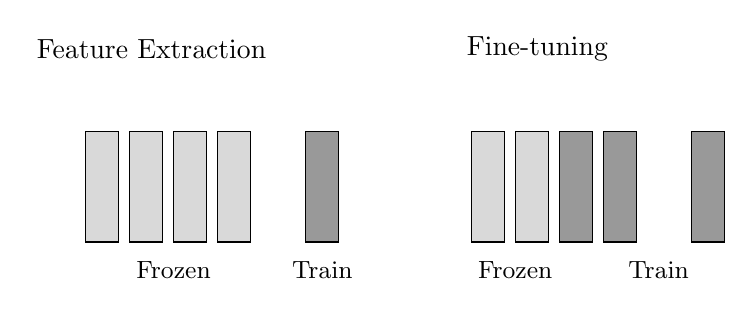
\begin{tikzpicture}[scale=0.7]
    % Feature extraction
    \begin{scope}
    \node at (2,3.5) {Feature Extraction};
    \foreach \i in {1,2,3,4} {
        \draw[fill=black!15] (\i*0.8,0) rectangle (\i*0.8+0.6,2);
    }
    \draw[fill=black!40] (4.8,0) rectangle (5.4,2);
    \node at (2.4,-0.5) {\small Frozen};
    \node at (5.1,-0.5) {\small Train};
    \end{scope}

    % Fine-tuning
    \begin{scope}[xshift=7cm]
    \node at (2,3.5) {Fine-tuning};
    \foreach \i in {1,2} {
        \draw[fill=black!15] (\i*0.8,0) rectangle (\i*0.8+0.6,2);
    }
    \foreach \i in {3,4} {
        \draw[fill=black!40] (\i*0.8,0) rectangle (\i*0.8+0.6,2);
    }
    \draw[fill=black!40] (4.8,0) rectangle (5.4,2);
    \node at (1.6,-0.5) {\small Frozen};
    \node at (4.2,-0.5) {\small Train};
    \end{scope}
\end{tikzpicture}
\caption{Left: freeze pre-trained layers, train only classifier. Right: fine-tune later layers too.}
\label{fig:transfer_strategies}
\end{figure}

\newthought{Feature extraction} freezes the pre-trained network and trains only a new classifier head. Fine-tuning unfreezes some or all layers and trains with a small learning rate. Full fine-tuning trains the entire network but risks catastrophic forgetting\index{catastrophic forgetting}.

\marginnote{\newthought{Fine-tuning vs.\ freezing.} When the target task is close to the source task, the backbone features can be used as-is (frozen). When the domains differ, fine-tuning the backbone with a small learning rate adapts the features while preserving the structure learned during pretraining.}

\subsection{When Transfer Fails}\index{negative transfer}

\newthought{Negative transfer} occurs when performance is worse than training from scratch. This happens when the source and target domains are very different, or when pre-trained features are harmful for the target task.


\subsection{Backbones and Pretraining Datasets}\index{backbone}

\marginnote{\newthought{A backbone} is an encoder trained on one task, then reused as a feature extractor for another. It supplies representations; a lightweight head on top supplies predictions.}

\newthought{Generalisation}\index{generalisation} is the reason transfer works.
A bottlenecked encoder must compress, and compression requires ignoring idiosyncratic noise in favour of shared structure.
A $k$-dimensional embedding with $k \ll d$ cannot memorise individual inputs; it must discover regularities that hold across the training distribution.
Those regularities, the semantic features, are precisely what a downstream model needs to perform well on new, unseen data.

\newthought{The quality of transferred features depends on the source dataset.}
A backbone is only as general as the data it was trained on.
Across domains, a small number of large-scale datasets have become the standard foundations for pretraining.

\begin{table*}[ht]
\centering
\begin{tabular}{p{0.14\textwidth}p{0.10\textwidth}p{0.10\textwidth}p{0.38\textwidth}}
    \toprule
    \textbf{Dataset} & \textbf{Modality} & \textbf{Scale} & \textbf{What the backbone learns} \\
    \midrule
    ImageNet \citealt{Deng2009ImageNet} & Images & 14M images & Edges, textures, object parts, and category-level semantics. The de facto starting point for visual feature extractors. \\
    The Pile \citealt{Gao2020Pile} & Text & 825 GB text & Syntax, coreference, factual associations, and discourse structure from books, academic papers, web text, and code. \\
    LibriSpeech \citealt{Panayotov2015LibriSpeech} & Audio & 1000 h audio & Phoneme boundaries, prosody, and speaker-invariant representations from read English speech. \\
    Kinetics-700 \citealt{Carreira2022Kinetics700} & Video & 650k clips & Temporal dynamics, motion patterns, and action semantics from short video clips spanning 700 human action classes. \\
    ShapeNet \citealt{Chang2015ShapeNet} & 3D shapes & 51k models & Surface geometry, part decomposition, and pose-invariant structure from annotated CAD models across 55 object categories. \\
    LAION-5B \citealt{Schuhmann2022LAION5B} & Image + text & 5.8B pairs & Joint visual and linguistic semantics from web-crawled image-caption pairs; the foundation behind open multimodal models. \\
    CheXpert \citealt{Irvin2019CheXpert} & Medical images & 224k X-rays & Anatomical landmarks, pathology signatures, and radiological texture patterns from labelled chest radiographs. \\
    ZINC \citealt{Sterling2015ZINC} & Molecular graphs & 250k molecules & Bond topology, functional-group motifs, and drug-likeness features from curated small-molecule structures. \\
    \bottomrule
\end{tabular}
\vspace{2em}
\caption{Large-scale pretraining datasets across modalities. Each dataset provides the raw material for a backbone to learn general-purpose features that transfer to downstream tasks within (and sometimes across) its modality.}
\label{tab:pretraining_datasets}
\end{table*}

\marginnote{\newthought{Modality matters.} An ImageNet backbone transfers well to satellite imagery or medical photos, but poorly to molecular graphs or audio spectrograms. Choosing the right source dataset and modality is the first design decision in any transfer learning pipeline.}


\section{Zero-Shot Learning}\index{zero-shot learning}

\marginnote{Zero-shot: classify without any training examples of that class.}

\newthought{Three families of approaches} exist. Attribute-based methods map classes to attributes and classify via attribute prediction. Embedding-based methods map both images and class names to a shared space. Generative methods synthesise features for unseen classes from descriptions.

\subsection{Vision-Language Alignment}

Modern zero-shot learning uses vision-language models:

\begin{equation}
    p(y = k | x) = \frac{\exp(\text{sim}(f_{\text{image}}(x), f_{\text{text}}(t_k)) / \tau)}{\sum_j \exp(\text{sim}(f_{\text{image}}(x), f_{\text{text}}(t_j)) / \tau)}
\end{equation}

where $t_k$ is the text description for class $k$.


\section{CLIP: Contrastive Language-Image Pre-training}\index{CLIP}

\marginnote{\newthought{CLIP.} Trained on 400M image-text pairs from the web~\cite{Radford2021CLIP}.}

\newthought{CLIP} consists of an image encoder, either ResNet or Vision Transformer, and a text encoder, a Transformer, trained jointly with a contrastive loss on image-caption pairs.

\begin{figure}
\centering
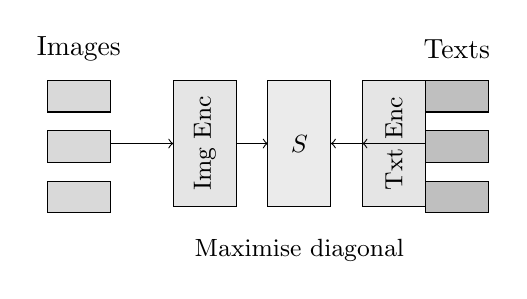
\begin{tikzpicture}[scale=0.8]
    % Images
    \node at (0,3) {Images};
    \foreach \i in {0,1,2} {
        \draw[fill=black!15] (-0.5,2-\i*0.8) rectangle (0.5,2.5-\i*0.8);
    }

    % Image encoder
    \draw[fill=black!10] (1.5,0.5) rectangle (2.5,2.5);
    \node[rotate=90] at (2,1.5) {\small Img Enc};

    % Text
    \node at (6,3) {Texts};
    \foreach \i in {0,1,2} {
        \draw[fill=black!25] (5.5,2-\i*0.8) rectangle (6.5,2.5-\i*0.8);
    }

    % Text encoder
    \draw[fill=black!10] (4.5,0.5) rectangle (5.5,2.5);
    \node[rotate=90] at (5,1.5) {\small Txt Enc};

    % Similarity matrix
    \draw[fill=black!8] (3,0.5) rectangle (4,2.5);
    \node at (3.5,1.5) {\small $S$};

    % Arrows
    \draw[->] (0.5,1.5) -- (1.5,1.5);
    \draw[->] (5.5,1.5) -- (4.5,1.5);
    \draw[->] (2.5,1.5) -- (3,1.5);
    \draw[->] (4.5,1.5) -- (4,1.5);

    % Diagonal
    \node at (3.5,-0.2) {\small Maximise diagonal};
\end{tikzpicture}
\caption{CLIP training: maximise similarity between matching image-text pairs along the diagonal.}
\label{fig:clip_training}
\end{figure}

\subsection{Zero-Shot Classification with CLIP}

\begin{algorithm}[H]
\caption{CLIP Zero-Shot Classification}
\begin{algorithmic}[1]
\Require Image $x$, class names $\{c_1, \ldots, c_K\}$, prompt template $T$
\For{each class $k$}
    \State $t_k \gets T(c_k)$ \Comment{e.g.\ ``a photo of a \{class\}''}
    \State $e_k \gets f_{\text{text}}(t_k)$ \Comment{Text embedding}
\EndFor
\State $e_x \gets f_{\text{image}}(x)$ \Comment{Image embedding}
\State $\hat{y} \gets \arg\max_k \cos(e_x, e_k)$
\end{algorithmic}
\end{algorithm}


\section{Prompt Engineering}\index{prompt engineering}

\marginnote{The prompt is the new hyperparameter.}

\newthought{The choice of text prompt} significantly affects performance:

\begin{table}
\centering
\begin{tabular}{lc}
\toprule
\textbf{Prompt} & \textbf{Accuracy} \\
\midrule
``\{class\}'' & 58.2\% \\
``a photo of a \{class\}'' & 63.5\% \\
``a photo of a \{class\}, a type of pet'' & 67.1\% \\
Ensemble of 80 prompts & 76.2\% \\
\bottomrule
\end{tabular}
\caption{Prompt engineering effects on ImageNet zero-shot accuracy.}
\label{tab:prompt_engineering}
\end{table}

\newthought{Prompt ensembling} averages embeddings from multiple prompt templates.

\newthought{CoOp}\index{CoOp} learns soft prompt tokens via gradient descent~\cite{Zhou2022CoOp}:
\begin{equation}
    t = [V_1][V_2]\ldots[V_M][\text{class}]
\end{equation}
where $V_i$ are learnable embeddings.


\section{Few-Shot Learning}\index{few-shot learning}

\marginnote{Few-shot: learn from 1--5 examples per class.}

\subsection{Fine-tuning Approaches}

\newthought{Linear probing}\index{linear probe} freezes the encoder and trains a linear classifier. Full fine-tuning updates all parameters but risks overfitting. Adapters\index{adapter} add small trainable modules while freezing the rest of the network.

\subsection{In-Context Learning}\index{in-context learning}

\newthought{Large language models} can do few-shot via prompting: provide a few input-output examples in the prompt, then query for a new input. No gradient updates are needed; the model learns from the examples in context.


\section{Foundation Models}\index{foundation model}

\marginnote{Foundation models: large pre-trained models that serve as building blocks.}

\subsection{SAM: Segment Anything Model}\index{SAM}

\newthought{SAM} was trained on 1 billion masks from 11 million images~\cite{Kirillov2023SAM}. It is promptable via point, box, or text input, and achieves zero-shot segmentation of arbitrary objects.

\subsection{DINO: Self-Distillation with No Labels}\index{DINO}

\newthought{DINO} is a self-supervised vision transformer~\cite{Caron2021DINO} that learns semantic features without any labels. Its attention maps highlight object parts, making the learned representations highly interpretable.

\subsection{Composing Foundation Models}

\newthought{Combining} CLIP for understanding, SAM for segmentation, and Stable Diffusion for generation enables complex pipelines without task-specific training.


\section{Domain Adaptation}\index{domain adaptation}

\marginnote{What if training and test data come from different distributions?}

\subsection{Types of Shift}

\newthought{Covariate shift}\index{covariate shift} occurs when $P(X)$ changes but $P(Y|X)$ stays the same. Label shift\index{label shift} occurs when $P(Y)$ changes but $P(X|Y)$ stays the same. Concept drift\index{concept drift} occurs when $P(Y|X)$ changes over time.

\subsection{Domain-Invariant Features}

\newthought{The goal} is to learn features that are informative for the task but indistinguishable between domains:

\begin{equation}
    \min_f \mathcal{L}_{\text{task}}(f) + \lambda \mathcal{L}_{\text{domain}}(f)
\end{equation}

where $\mathcal{L}_{\text{domain}}$ penalises features that reveal domain identity.

\subsection{Adversarial Domain Adaptation}\index{adversarial domain adaptation}

\newthought{An adversarial approach} trains a domain discriminator; the encoder tries to fool it~\cite{Ganin2016DomainAdversarial}:

\begin{figure}
\centering
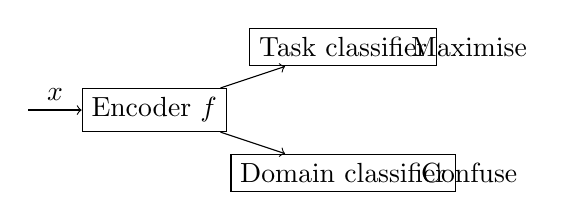
\begin{tikzpicture}[scale=0.8]
    \node[draw, rectangle] (enc) at (0,0) {Encoder $f$};
    \node[draw, rectangle] (task) at (3,1) {Task classifier};
    \node[draw, rectangle] (domain) at (3,-1) {Domain classifier};

    \draw[->] (-2,0) -- (enc) node[midway, above] {$x$};
    \draw[->] (enc) -- (task);
    \draw[->] (enc) -- (domain);

    \node at (5,1) {Maximise};
    \node at (5,-1) {Confuse};
\end{tikzpicture}
\caption{Adversarial domain adaptation: features should help the task but not reveal the domain.}
\label{fig:domain_adaptation}
\end{figure}


%═══════════════════════════════════════════════════════════════════════
% BLOCK 3: STUDENT ACTIVATION
%═══════════════════════════════════════════════════════════════════════

\newpage
\section{Examples \& Exercises}

\subsection{Exercise 1: Zero-Shot with CLIP}

You want to classify images into \{beach, mountain, city, forest\}.

\begin{enumerate}
    \item Write 3 different prompt templates.
    \item How would you ensemble them?
    \item What if ``forest'' and ``mountain'' are often confused?
\end{enumerate}

\subsection{Exercise 2: Few-Shot Fine-tuning}

You have 5 examples per class for a 10-class problem, 50 examples total.

\begin{enumerate}
    \item Why might full fine-tuning fail?
    \item What regularisation would you use?
\end{enumerate}

\subsection{Exercise 3: Domain Shift}

Your model trained on ImageNet performs poorly on medical X-rays.

\begin{enumerate}
    \item What type of domain shift is this?
    \item Propose two solutions.
\end{enumerate}


\section{Self-Reflection and Recap}

\newthought{Self-Reflection.}

\begin{enumerate}
    \item Why does CLIP generalise to unseen categories?
    \item When does fine-tuning outperform zero-shot, and when is the reverse true?
    \item How does prompt ensembling reduce the sensitivity to a single prompt choice?
    \item What makes CoOp's learned prompts more effective than hand-crafted ones?
    \item When would you prefer a linear probe over full fine-tuning for few-shot tasks?
    \item How does adversarial domain adaptation differ from simply fine-tuning on target data?
    \item What risks arise when composing multiple foundation models in a pipeline?
\end{enumerate}

\vspace{1.5em}

\newthought{Recap.}

\begin{itemize}
    \item Transfer learning reuses pre-trained features; early layers transfer well, but late layers require adaptation, and large domain gaps risk negative transfer.
    \item Zero-shot classification via CLIP matches image embeddings to text prompt embeddings; prompt design and ensembling are critical for accuracy.
    \item Few-shot strategies range from linear probing to full fine-tuning; the right choice depends on how much labelled data is available and how far the target domain is from the source.
    \item Domain adaptation techniques learn features that are informative for the task but invariant to the domain, mitigating covariate shift.
    \item Foundation models such as CLIP, SAM, and DINO serve as composable building blocks for tasks they were never explicitly trained on.
\end{itemize}

\vspace{2.5em}

\marginnote{\newthought{Teaser.} What if we have labels, but they are noisy, partial, or generated by heuristics rather than experts?}

\newthought{We have seen models that work without labels.} But in practice, we often have labels that are imperfect: noisy crowd annotations, heuristic rules, and biased labellers are the reality of real-world data.

\newthought{The next chapter explores weak supervision,} where multiple noisy labelling functions are combined into a probabilistic label model, and training proceeds despite imperfect supervision.

\marginnote{\newthought{feedback}}
